	Acerca do projeto da bancada de testes não destrutivos para amortecedores de carros populares, descreve-se a seguir as definições de projeto da área de energia.

	\textbf{Objetivo Geral}

	Acionar o sistema de teste de amortecedores por meio do motor de indução trifásico, dimensionado a partir dos dados da carga requerida pelo teste, bem como controlar as velocidades exigidas, através do inversor de frequência. Monitorar a temperatura do fluido dentro do amortecedor através do gradiente de temperatura obtido em simulações realizadas nos softwares Ansys e MATLAB.

	\textbf{Objetivos Específicos}

	\begin{itemize}
		\item Dimensionamento do conjunto motor/inversor e de seus componentes;
		\item Definição do sistema de proteção;
		\item Construção dos circuitos de acionamento, proteção e controle;
		\item Definição do tipo de controle e dos parâmetros programados no inversor de frequência;
		\item Análise e definição da forma de programação necessária para a integração eletrônica com o inversor;
		\item Estudo da possibilidade de monitorar a temperatura do fluido existente no interior do amortecedor testado.
	\end{itemize}

	\textbf{EAP}

	\begin{figure}[!h]
		\centering
		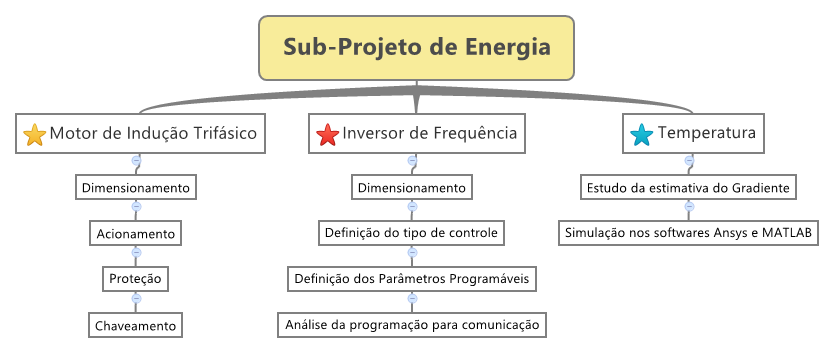
\includegraphics[scale=0.5]{eap-energia.png}
		\caption{Estrutura Analítica do Projeto de Energia}
		\label{eap-energia}
	\end{figure}

	Nos parágrafos a seguir descreve-se brevemente os pacotes de trabalho apresentados na EAP do projeto de energia. 

	\textit{Motor de indução trifásico}:


	- Sistema de acionamento e proteção do motor: aciona com segurança e protege o motor trifásico contra elevados níveis de tensão e corrente.

	- Chaveamento: aciona o motor e estabelece as velocidades, por meio da comunicação com o inversor de frequência.

	\textit{Inversor de frequência}:

	
	- Parâmetros de controle programados no inversor: a programação dos parâmetros de controle definem as características de operação do motor.
	
	- Acionamento e controle da velocidade do motor: aciona e controla com precisão as velocidades que o motor entregará ao sistema.

	\textit{Controle de temperatura}:

	
	- Gradiente de temperatura do fluido dentro do amortecedor: com o gradiente de temperatura é possível descrever e monitorar a temperatura do fluido dentro do amortecedor durante os testes, fazendo com que haja um controle preciso da temperatura.
	
	- Simulações nos softwares Ansys e MATLAB: com as simulações realizadas nestes softwares será obtido o gradiente de temperatura que descreverá a temperatura do fluido do amortecedor a partir da temperatura da superfície do mesmo durante os testes realizados.

	\textbf{Lista É / Não É}

	\textit{ É função da equipe do projeto de Energia:}

	\begin{itemize}
		\item Acionar o sistema de teste de amortecedores utilizando um motor elétrico;
		\item Controlar as velocidades do teste por meio de um inversor de frequência;
		\item Dimensionar o conjunto motor/inversor;
		\item Construir os circuitos de acionamento, proteção e controle;
		\item Definir o tipo de controle e a programação dos parâmetros do inversor de frequência;
		\item Definir a forma de conexão do inversor de frequência com a eletrônica (em conjunto com a equipe da eletrônica);
		\item Estudar as formas de monitorar a temperatura do fluido do amortecedor.
	\end{itemize}

	\textit{ Não é função da equipe do projeto de Energia:}

	\begin{itemize}
		\item Dimensionar e definir o sistema de transmissão;
		\item Dimensionar e definir o sistema biela manivela;
		\item Dimensionar e estabelecer dados da carga requerida no teste.

	\end{itemize}

	\textbf{Requisitos}

	O conjunto motor/inversor dimensionado deve atender o torque solicitado e realizar o controle das diferentes velocidades solicitadas pelo usuário. O gradiente de temperatura obtido nas simulações realizadas nos softwares Ansys e MATLAB deve descrever corretamente a temperatura do fluido dentro do amortecedor durante a realização dos testes, a partir da temperatura da superfície do amortecedor medida, permitindo uma análise completa do amortecedor e de suas características.

	\begin{itemize}
		\item O motor deve atender corretamente as exigências do sistema;
		\item O inversor de frequência deve colaborar com o acionamento do motor e fazer o controle correto das velocidades exigidas no teste;
		\item  O gradiente de temperatura do fluido deve ser estimado através das simulações realizadas nos softwares Ansys e MATLAB.
	\end{itemize}

	\textbf{Propósito}

	Será utilizado um motor de indução trifásico, visto que o mesmo possui as características suficientes para atender o sistema, além de ser um motor de fácil manuseio e possibilitar o uso de um inversor de frequência, que tem o controle mais preciso da velocidade do motor. A obtenção do gradiente de temperatura do fluido dentro do amortecedor através de simulações realizadas nos softwares Ansys e MATLAB será algo inovador, pois os testes atuais em amortecedores medem apenas a temperatura da superfície dos mesmos, além de ser de suma importância, visto que a temperatura do fluido influencia diretamente na eficiência do amortecedor.

	\textbf{Cronograma}

	A Tabela \ref{cronogramaenergia} mostra o cronograma desenvolvido em termos das macros do projeto de energia.

	\newpage
	\begin{table}[!h]
		\centering
		\caption{Cronograma de macros do projeto de energia}
		\label{cronogramaenergia}
		\resizebox{\textwidth}{!}{%
		\begin{tabular}{lccc}
		\hline
		\rowcolor[HTML]{C0C0C0} 
		\textbf{ATIVIDADE} & \textbf{DATA DE INÍCIO/FIM} & \textbf{RESPONSÁVEL} & \textbf{(\%) COMPLETO} \\ \hline
		Dimensionamento do conjunto motor/inversor & 04/04 - 10/04 & \begin{tabular}[c]{@{}c@{}}Ana Rafaela,\\ Ludmila\end{tabular} & 100\% \\ \hline
		\begin{tabular}[c]{@{}l@{}}Estudo das possibilidades de execução dos\\ testes no motor e inversor\end{tabular} & 10/04 - 20/04 & \begin{tabular}[c]{@{}c@{}}Ana Rafaela,\\ Ludmila\end{tabular} & 100\% \\ \hline
		\begin{tabular}[c]{@{}l@{}}Estudo dos tipos de controle e dos parâmetros\\ programáveis no inversor de frequência\end{tabular} & 20/04 - 25/05 & \begin{tabular}[c]{@{}c@{}}Ana Rafaela,\\ Ludmila,\\ Micaelle\end{tabular} & 100\% \\ \hline
		\begin{tabular}[c]{@{}l@{}}Execução de testes a vazio e com carga\\ no motor\end{tabular} & 02/05 - 20/05 & \begin{tabular}[c]{@{}c@{}}Ana Rafaela,\\ Ludmila,\\ Micaelle,\\ Thialei\end{tabular} & 100\% \\ \hline
		\begin{tabular}[c]{@{}l@{}}Estudo sobre as propriedades do fluido\\ dentro do amortecedor e sobre a possibilidade\\ de monitorar essa temperatura\end{tabular} & 29/04 - 19/05 & \begin{tabular}[c]{@{}c@{}}Micaelle,\\ Thialei\end{tabular} & 100\% \\ \hline
		\begin{tabular}[c]{@{}l@{}}Novos testes no acionamento do motor e\\ controle de velocidades\end{tabular} & 30/05 - 03/06 & \begin{tabular}[c]{@{}c@{}}Ana Rafaela,\\ Ludmila\end{tabular} & 1000\% \\ \hline
		\begin{tabular}[c]{@{}l@{}}Monitorar a elevação de temperatura do\\ motor para o tempo de teste demandado\end{tabular} & 06/04 - 10/05 & \begin{tabular}[c]{@{}c@{}}Micaelle,\\ Thialei\end{tabular} & 0\% \\ \hline
		\begin{tabular}[c]{@{}l@{}}Simulação do gradiente de temperatura do\\ fluido do amortecedor\end{tabular} & 20/05 - 23/06 & \begin{tabular}[c]{@{}c@{}}Micaelle,\\ Thialei\end{tabular} & 0\% \\ \hline
		\begin{tabular}[c]{@{}l@{}}Testes de Amortecedores com\\ estrutura adaptada\end{tabular} & 20/05 - 23/06 & \begin{tabular}[c]{@{}c@{}}Ana Rafaela,\\ Ludmila\end{tabular} & 100\% \\ \hline
		\end{tabular}%
		}
	\end{table}

	\textbf{Investimento}

	A tabela \ref{investimentoenergia} apresenta uma descrição preliminar do investimento projetado ao longo do projeto para aquisição de componentes do projeto de energia.

	\begin{table}[!h]
		\centering
		\caption{Investimento do Projeto de Energia}
		\label{investimentoenergia}
		\resizebox{\textwidth}{!}{%
		\begin{tabular}{|c|c|c|c|c|c|}
		\hline
		\rowcolor[HTML]{C0C0C0} 
		\textbf{N} & \textbf{Item} & \textbf{Valor (R)} & \textbf{Quantidade} & \textbf{\begin{tabular}[c]{@{}c@{}}Data da\\ Compra\end{tabular}} & \textbf{Objetivo} \\ \hline
		1 & Motor trifásico & 0,00 & 1 & - & Acionar o sistema \\ \hline
		2 & Inversor de frequência & 0,00 & 1 & - & \begin{tabular}[c]{@{}c@{}}Controlar a velocidade\\ do motor\end{tabular} \\ \hline
		3 & Fusível de 16A & 0,00 & 1 & - & Proteger o motor e inversor \\ \hline
		4 & Chave seletora & 0,00 & 1 & - & \begin{tabular}[c]{@{}c@{}}Acionamento do motor e\\ das diferentes velocidades\end{tabular} \\ \hline
		5 & Fios & 0,00 & 1 & - & \begin{tabular}[c]{@{}c@{}}Fazer as ligações entre o motor,\\ o inversor e o sistema de\\ acionamento e\\ proteção\end{tabular} \\ \hline
		6 & Acoplamento & 54,00 & 1 & 15/05 & Acoplar os motores para teste \\ \hline
		7 & Serviço do torneador & 65,00 & 1 & 16/05 & Furar o acoplamento \\ \hline
		8 & Freio de Prony & 0,00 & 1 & - & Simular carga no eixo do motor \\ \hline
		9 & \begin{tabular}[c]{@{}c@{}}Estrutura de fixação\\ do freio na,bancada\end{tabular} & 0,00 & 1 & - & \begin{tabular}[c]{@{}c@{}}Fixar o sistema do freio de\\ Prony junto com o motor\end{tabular} \\ \hline
		\end{tabular}%
		}
	\end{table}


	\textbf{Restrições e Riscos}

	A restrição de gastos imposta ao grupo, de certa forma, restringiu a definição do conjunto motor/inversor, visto que se trata de elementos de elevado custo. A montagem e operação do sistema elétrico oferecem riscos como choques elétricos e danos aos equipamentos diante de situações mal executadas e não utilização de equipamentos de proteção. Existe a possibilidade de não se obter êxito nas simulações que serão realizadas nos softwares Ansys e MATLAB para a obtenção do gradiente de temperatura do fluido dentro do amortecedor.

	\textbf{Milestones Identificadas}

	A Tabela \ref{milestones-energia} apresenta as milestones identificadas para o projeto.
	\begin{table}[!hptb]
		\centering
		\caption{Milestones do Projeto de Energia}
		\label{milestones-energia}
		\begin{tabular}{|l|c|}
		\hline
		\rowcolor[HTML]{C0C0C0} 
		\multicolumn{1}{|c|}{\cellcolor[HTML]{C0C0C0}{\color[HTML]{000000} \textbf{Produto}}} & {\color[HTML]{000000} \textbf{Entregue em}} \\ \hline
		{\color[HTML]{000000} Apresentação de formas de acionar o sistema.} & {\color[HTML]{000000} Ponto de controle 1} \\ \hline
		{\color[HTML]{000000} \begin{tabular}[c]{@{}l@{}}Definição da máquina a ser utilizada, dos sistemas, \\ de acionamento, proteção e forma de controle de velocidade.\end{tabular}} & {\color[HTML]{000000} Ponto de controle 2} \\ \hline
		{\color[HTML]{000000} Montagem do sistema de acionamento e proteção do,motor.} & {\color[HTML]{000000} Ponto de controle 2} \\ \hline
		{\color[HTML]{000000} \begin{tabular}[c]{@{}l@{}}Testes de acionamento do motor (a vazio e com\\ carga),com o inversor de frequência.\end{tabular}} & {\color[HTML]{000000} Ponto de controle 2} \\ \hline
		{\color[HTML]{000000} \begin{tabular}[c]{@{}l@{}}Estudo de simulações nos softwares Ansys e MATLAB,\\ para a obtenção do gradiente de temperatura do fluido.\end{tabular}} & {\color[HTML]{000000} Ponto de controle 2} \\ \hline
		{\color[HTML]{000000} \begin{tabular}[c]{@{}l@{}}Testes com Amortecedores com estrutura adaptada.\end{tabular}} & {\color[HTML]{000000} Ponto de controle 3} \\ \hline
		\end{tabular}
	\end{table}

\subsection{Ponto de Controle II}
\subsubsection{Dimensionamento do Conjunto Motor/Inversor}

	A definição do motor a ser utilizado no teste de amortecedores foi baseada, inicialmente, para fins de conhecimento do sistema, nas literaturas \cite{Duarte}\cite{Vandresen} semelhantes à aplicação em questão e, posteriormente, para fins de cálculos e dimensionamento, aos dados requeridos pela carga durante o teste. 
	
	Diante do estudo das características da carga a ser acionada, que, por se tratar de um sistema de excitação de um amortecedor automotivo, tem um comportamento variável no que diz respeito à força, quando se varia a velocidade exigida \cite{Duarte}, foi possível definir o motor a ser utilizado. Além disso, a partir da necessidade de se alterar velocidades durante o teste, foi definido o uso de um inversor de frequência para realizar o controle da velocidade do motor.
	
	Dos dados da carga e do sistema de transmissão que compõem a bancada, foi possível estimar que a maior potência exigida ao motor foi de aproximadamente 0,37 cavalo-vapor (cv). Com isso, a definição do motor foi realizada e a Tabela abaixo mostra as características de desempenho do mesmo.

	\newpage
	\begin{figure}[!h]
		\centering
		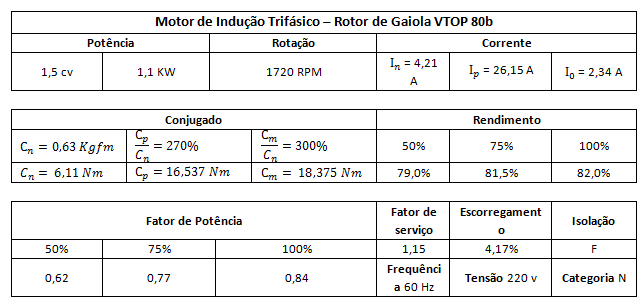
\includegraphics[scale=0.9]{motorEspecificacao.png}
		\caption[Características de desempenho do motor]{Características de desempenho do motor \cite{Voges}}
		\label{motorEspecificacao}
	\end{figure}

	A fim de se verificar a viabilidade de aplicação do motor para a excitação do sistema, inicialmente, foram feitos os seguintes cálculos, baseados nas Equações abaixo \cite{Chapman}:

	- \textbf{Velocidade síncrona} :

	$$ n_{sinc} = \frac{120f_{se}}{p} = \frac{120*60Hz}{4 polos} = 1800rpm $$

	- \textbf{Velocidade do rotor} :

	$$ n_{m} = (1 - s)n_{sinc} = (1 - 0,00417) * 1800rpm = 1724,94rpm $$

	- \textbf{Frequência do rotor} :

	$$ f_{re} = sf_{se} = 0,00417 * 60Hz = 2,5Hz $$

	- \textbf{Conjugado de carga no eixo} :

	$$ \tau_{carga} = \frac{P_{saída}}{\omega_{m}} = \frac{1,5cv * 735,5W}{1724,94rpm * 2\pi/60} = 6,11 N.m $$

	O controle de velocidade que se faz necessário no teste foi definido para ser executado através de um inversor de frequência, como já mencionado, que, além de permitir uma faixa razoável de variação na velocidade, dependente do tipo de controle utilizado, permite ainda a adaptação do sistema de acionamento do motor em relação às características de operação da carga.
	
	O dimensionamento de um inversor de frequência deve ser feito em função da corrente nominal do motor utilizado, que deve ser menor ou igual à corrente nominal de saída do inversor \cite{WEGIF}. Portanto, o inversor, cujas características estão explicitadas na tabela abaixo, é compatível ao motor utilizado.

	- \textbf{Dados do Inversor}:

	\begin{figure}[!h]
		\centering
		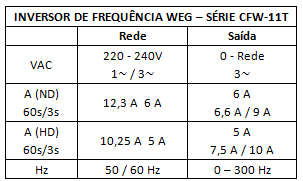
\includegraphics[scale=1]{caractMotor.png}
		\caption[Características do inversor]{Características do inversor \cite{WEGIF}}
		\label{caractMotor}
	\end{figure}

	O MIT utilizado possui uma característica muito importante a nível de dimensionamento: sua autoventilação. Esse fato implica limitações no desempenho do motor quando este precisa operar a baixas velocidades, onde ocorre uma redução na ventilação, sendo necessária uma diminuição no torque demandado, de modo a manter a temperatura dentro dos limites térmicos exigidos \cite{WEGMotorEletrico}.

	É possível então definir a faixa de operação do motor quanto aos valores de torques e suas respectivas velocidades, garantindo uma margem de segurança durante todo o trabalho do conjunto motor/inversor. A partir do gráfico abaixo, o qual expressa o fator de redução do torque (“derating factor”) para motores autoventilados, levando em consideração as influências da redução da ventilação em baixas rotações, foi possível obter os valores a serem fornecidos durante o teste.

	\newpage
	\begin{figure}[!h]
		\centering
		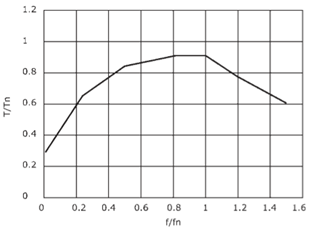
\includegraphics[scale=1]{graficoRT4.png}
		\caption[Curva torque x frequência para motores fechados, auto-ventilados]{Curva torque x frequência para motores fechados, auto-ventilados \cite{WEGIF}}
		\label{graficoRT4}
	\end{figure}

	As equações correspondentes a cada trecho da curva da figura \ref{graficoRT4} são as seguintes:

	Frequência normalizada $f_{r}$, dada pela razão entre frequência de operação $f$ e frequência nominal $f_{n}$:

	$$ f_{r} = \frac{f}{f_{n}} $$

	Para 0 $\leq f_{r}$ < 0,25:

	$$ \frac{T}{T_{n}} = (1,49*f_{r}) + 0,28 $$

	Para 0,25 $\leq f_{r}$ < 0,50:

	$$ \frac{T}{T_{n}} = (0,74*f_{r}) + 0,47 $$

	Para 0,50 $\leq f_{r}$ < 0,83:

	$$ \frac{T}{T_{n}} = (0,28*f_{r}) + 0,70 $$

	Para 0,83 $\leq f_{r}$ < 1:

	$$ \frac{T}{T_{n}} = 0,93 $$

	Para $f_{r}$ > 1:
	
	$$ \frac{T}{T_{n}} = \frac{0,93}{f_{r}} $$


	Diante do pressuposto que o dimensionamento do motor deve ser executado a partir da pior situação de funcionamento exigida \cite{WEG03}, será analisado então, a partir das possibilidades de teste no amortecedor, o caso simulado onde será exigida uma velocidade no motor de 679,54 rpm, que se mostra como o caso mais crítico de operação do mesmo, onde, através do sistema de redução, será possível atingir a velocidade mínima requerida pelo teste. Para tal velocidade, foi feito um teste (que se encontra detalhado no tópico “Aplicação – Ensaios de laboratório” abaixo) com o motor inicialmente a vazio, sendo possível simular que, para a velocidade de 679 rpm no rotor, deveria ser programada uma velocidade de 700 rpm no inversor de frequência. Essa diferença de velocidades acontece devido ao escorregamento existente, sendo que com esses valores, foi possível calcular o escorregamento para tal situação. Seguem os cálculos embasados na curva torque x frequência para motores auto-ventilados explicitada acima.

	$$ s = \frac{n_{s} - n_{r}}{n_{s}} = \frac{700 - 679,54}{700} = 0,029 $$

	$$ f = \frac{n * p}{120} = \frac{679,54 rpm * 4 polos}{120} = 22,65 Hz $$

	$$ f_{r} = \frac{f}{f_{n}} = \frac{22,65 Hz}{60 Hz} = 0,38 $$

	$$ \frac{T}{T_{n}} = (0,74 * f_{r}) + 0,47 $$

	$$ \frac{T}{6,1 N.m} = 0,75 $$

	$$ T = 4,58 N.m $$

	Analisando esse resultado, diante da necessidade de acionamento da carga por um torque de 2,91 Nm, percebe-se que, mesmo considerando os valores mais críticos de teste, o motor ainda supera o torque demandado pela carga com um bom fator de segurança. Sendo assim, quando consideradas as possíveis perdas na caixa de redução, nas correias, nos rolamentos dos mancais da manivela, entre outras, que poderão exigir um pouco mais de força do motor, o fator de segurança existente entre o torque entregue pelo motor e o torque exigido pela carga, garantirá o bom funcionamento do sistema. Além disso, será feita por meio do inversor de frequência a compensação de escorregamento, fazendo com que seus valores não variem diante da variação de velocidade, adquirida pela imposição de carga no motor.

	Como os outros casos exigidos pelo teste são todos para velocidades acima de 679,54 rpm e para torques menores que 2,91 Nm, é seguro afirmar que o motor atenderá as solicitações do teste.


\subsubsection{Aplicação - Testes}
		
	\subsubsubsection{Ensaio a Vazio}

		A fim de se comprovar o comportamento inicial do conjunto motor/inversor, definir os parâmetros a serem programados, bem como apresentar o funcionamento do sistema para todo o grupo e facilitar o entendimento da comunicação com as demais áreas do projeto, foi feita a prática de acionamento do MIT a vazio com inversor de frequência.

		Foram utilizados os seguintes equipamentos:

		\begin{itemize}
			\item Motor de Indução Trifásico - Rotor de Gaiola VTOP 80b, Potência 1,5 cv;
			\item Inversor de Frequência (placa P009);
			\item 3 fusíveis de 16A (placa P012);
			\item 3 chaves seletoras (placa P011). 
		\end{itemize}

		As ligações feitas entre o motor e o inversor estão representadas no diagrama de montagem (circuito elétrico) abaixo:

		\newpage
		\begin{figure}[!h]
			\centering
			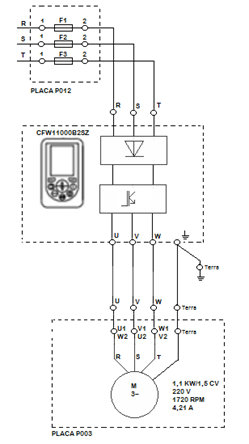
\includegraphics[scale=1]{diagramaEE01.png}
			\caption{Diagrama de montagem – circuito elétrico de acionamento do motor com inversor de frequência} 
			\label{diagramaEE01}
		\end{figure}

		Foi utilizado para esse teste o controle V/f do inversor, onde a programação dos seus parâmetros foi feita de forma que o controle de velocidades fosse realizado por um conjunto de posições de três chaves seletoras, sendo que, para cada posição, foi programada uma determinada velocidade. 

		Essa forma de controle foi apresentada de forma a colaborar com a integração eletrônica, visto que a apresentação do funcionamento do sistema utilizando as chaves seletoras facilitou o entendimento de como poderia ser feita a comunicação eletrônica com o inversor de frequência.

		\newpage
		\begin{figure}[!h]
			\centering
			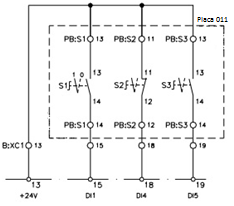
\includegraphics[scale=1]{diagramaEE02.png}
			\caption[Diagrama de montagem - chaves seletoras conectadas ao inversor]{Diagrama de montagem - chaves seletoras conectadas ao inversor \cite{WEGIF}} 
			\label{diagramaEE02}
		\end{figure}

		A lógica programada para as chaves seletoras pode ser analisada do ponto de vista dos números binários. Ao impor a condição de que a alimentação para o motor seria fornecida pelo acionamento da chave S1, a mesma sempre deveria estar na posição 1 para que o motor girasse. A mesma lógica numérica seguiu para as outras chaves, onde se programou segundo a imagem a seguir as seguintes posições e seguintes velocidades respectivas.

		\begin{figure}[!h]
			\centering
			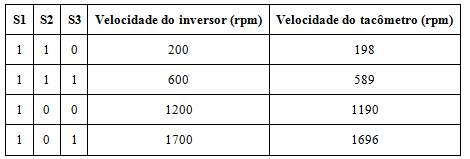
\includegraphics[scale=1]{posicaoChave.png}
			\caption[Posição das chaves de acionamento da velocidades programas com inversor]{Posição das chaves de acionamento da velocidades programas com inversor} 
			\label{posicaoChave}
		\end{figure}

	\subsubsubsection{Ensaios com Simulação de Cargas}

		\begin{itemize}
		\item \textbf{Gerador de Indução}
		\end{itemize}

			Como forma de comprovar o desempenho do MIT diante de cargas acopladas ao seu eixo, foi feita uma simulação utilizando um gerador de indução conectado à rede elétrica, onde o rotor da máquina de indução deveria ter velocidade superior à velocidade síncrona, para gerar energia \cite{Nascimento}. Seguindo essa teoria, é possível fazer com que a máquina opere como gerador quando a velocidade do rotor ultrapassa a velocidade síncrona, resultando tanto um escorregamento negativo quanto produzindo um torque também negativo.
			
			Para tal prática, deve-se adicionar um banco de capacitores que forneça energia reativa ao gerador de indução, que, por sua vez, consegue produzir energia de forma isolada, conforme elucida o esquema abaixo.

			\begin{figure}[!h]
				\centering
				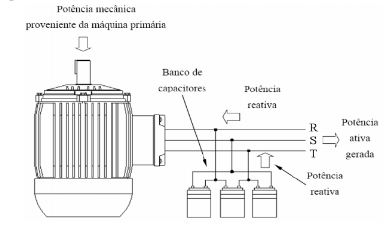
\includegraphics[scale=1]{diagramaEE03.png}
				\caption[Diagrama de ligação do banco de capacitores à máquina]{Diagrama de ligação do banco de capacitores à máquina \cite{Nascimento}} 
				\label{diagramaEE03}
			\end{figure}

			Para tal experimento, foram utilizados os seguintes equipamentos:

			\begin{itemize}
				\item 2 Motores de Indução Trifásico - Rotor de Gaiola VTOP 80b, Potência 1,5 cv;
				\item Inversor de Frequência (placa P009);
				\item 3 fusíveis de 16A (placa P012);
				\item 3 chaves seletoras (placa P011);
				\item Banco de 3 capacitores ligados em delta;
			\end{itemize}

			A bancada foi então disposta como mostra a figura \ref{bancadaEE}, onde mostra a ligação de todos os compenentes.

			\begin{figure}[!htpb]
				\centering
				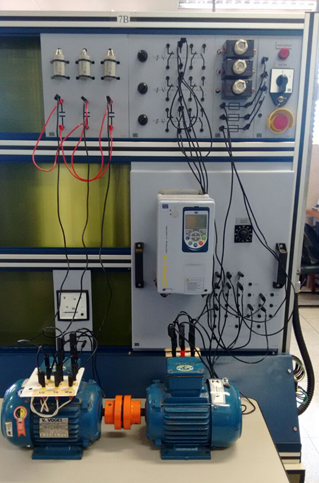
\includegraphics[scale=0.6]{bancadaEE.png}
				\caption[Circuito montado do acoplamento de dois motores]{Circuito montado do acoplamento de dois motores} 
				\label{bancadaEE}
			\end{figure}

			\newpage
			Por motivos ainda em fase de identificação, esse teste não obteve êxito. Apesar do dimensionamento do banco de capacitores ter sido feito de forma correta, baseado em literatura \cite{Vanco}, pode ser possível dizer que a simulação a baixas velocidades (de 600 a 1200 rpm), que são as velocidades de operação do motor para o teste demandado, não tenha permitido a ação do gerador de indução. Pretende-se, então, aprofundar os estudos quanto à possibilidade de execução desse teste a baixas velocidades, de forma a obter os resultados esperados.

		\begin{itemize}
		\item \textbf{Freio de Prony}
		\end{itemize}

			A outra forma de simulação de carga no motor foi através de um freio mecânico, conhecido como Freio de Prony, conforme a figura \ref{bancadaProny}.

			\begin{figure}[!hptb]
				\centering
				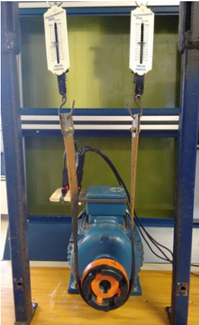
\includegraphics[scale=0.75]{bancadaProny.png}
				\caption[Freio de Prony acoplado ao motor]{Freio de Prony acoplado ao motor} 
				\label{bancadaProny}
			\end{figure}

			Iniciou-se o teste sem carga e foi esperado um tempo até que a velocidade do motor se estabilizasse. Logo após, foram adicionados incrementos de carga no freio, de forma manual, através das balanças analógicas utilizadas. A princípio, o ensaio foi meramente experimental, e, diante da ausência de equipamentos que permitissem a medição do torque para cada situação de carga e velocidade impostas, foi possível medir apenas a rotação no eixo do motor através de um tacômetro. Caso seja alcançado o objetivo de se fazer o experimento com células de carga, a medição precisa do torque se tornará possível.

			É importante ressaltar que foi perceptível durante esse ensaio que a variação de cargas no eixo do motor levou a quedas consideráveis de rotação. Para solucionar esse problema, foi utilizado o conceito de compensação de escorregamento, programado no inversor de frequência (controle V/f), que é responsável por incrementar a frequência de saída em função do aumento da corrente ativa do motor. Essa forma de controle (V/f) escolhida atende de forma satisfatória as necessidades de operação do motor para o teste de amortecedores, sendo que nos fornece a opção de manter a velocidade constante diante de variações na carga.  A programação desse parâmetro é importante, pois geralmente, para cada curso (compressão e tração) do teste de um amortecedor, tem-se uma força maior para um movimento e uma força menor para o outro, sendo que esse fator depende do tipo de amortecedor testado. Considerando a possibilidade dessa variação de força em uma mesma velocidade de teste, não são viáveis variações da velocidade programada para o motor, pois poderá afetar todo o sistema, alterando os resultados esperados.
			
			Para o ajuste do parâmetro que permite essa compensação, o motor foi acionado a vazio a 900 rpm, essa velocidade foi medida no eixo do motor por meio do tacômetro, obtendo-se o valor de 897,3 rpm, depois foi aplicada uma carga e o parâmetro foi incrementado até a velocidade atingir o mesmo valor do teste a vazio, sendo que todas as outras velocidades acionadas após a programação desse parâmetro tiveram automaticamente o mesmo comportamento.

			A figura \ref{resultadoEE01} mostra os resultados do teste.

 			\begin{figure}[!h]
				\centering
				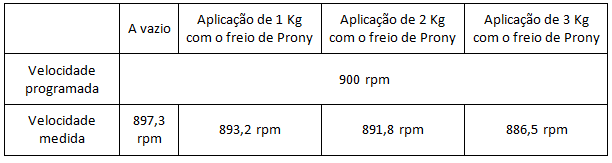
\includegraphics[scale=1]{resultadoEE01.png}
				\caption[Dados obtidos experimentalmente para motor a vazio com controle de inversor de frequência]{Dados obtidos experimentalmente para motor a vazio com controle de inversor de frequência} 
				\label{resultadoEE01}
			\end{figure}

			Após essas medições, a compensação então foi feita tendo como base a força de 30 Newtons, que para um raio de 4,2 cm (raio do acoplamento por onde passava a correia), tem-se como torque o valor de 1,26 Nm, obtendo-se os seguintes resultados:

			\begin{figure}[!h]
				\centering
				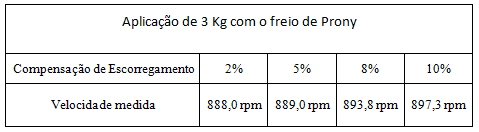
\includegraphics[scale=1]{resultadoEE02.png}
				\caption[Dados obtidos experimentalmente, motor com carga com o controle do inversor de frequência]{Dados obtidos experimentalmente, motor com carga com o controle do inversor de frequência} 
				\label{resultadoEE02}
			\end{figure}

			De acordo com os resultados, foi possível concluir que, ao incrementar o parâmetro de compensação de escorregamento, é possível manter a velocidade constante no teste, mesmo quando sujeito a variações de carga.

			\begin{figure}[!h]
				\centering
				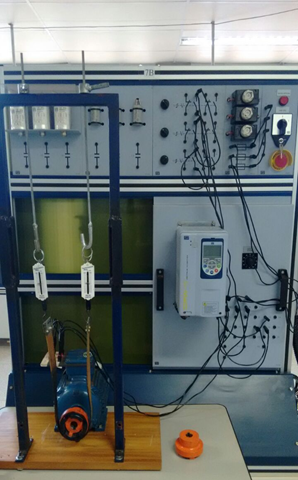
\includegraphics[scale=1]{bancadaEE02.png}
				\caption[Circuito para teste do torque do motor, com o princípio do mecanismo de Prony]{Circuito para teste do torque do motor, com o princípio do mecanismo de Prony} 
				\label{bancadaEE02}
			\end{figure}

			Depois da confirmação da funcionalidade de tal parâmetro, foi feito o teste aplicando uma força aproximada de 70 Newtons no eixo do motor, com um respectivo torque de 2,94 Nm (torque máximo exigido para o teste de amortecedor, a uma velocidade aproximada de 679,54 rpm). O teste foi feito com o motor funcionando durante 5 minutos, que é equivalente à realização de aproximadamente 52 ciclos no amortecedor a uma velocidade de 679 rpm no motor. Comprovou-se então que a velocidade de 679 rpm se manteve constante com a variação de carga, o comportamento do motor foi compatível ao esperado durante o ensaio e a situação mais crítica que será exigida pelo teste de amortecedor foi simulada e comprovada com segurança, dando assim maior confiabilidade para qualquer das outras situações exigida a partir dessa.

\subsubsection{Simulação Computacional de Transferência de Calor em Amortecedores}

	O estudo de transferência de calor entre diferentes superfícies de características distintas exige um rigor matemático na área de escoamento de fluidos, como é caso dos amortecedores. Os amortecedores possuem fluidos distintos e podem se comportar de maneiras diferentes diante de variações de temperatura.
	
	Algumas das equações envolvidas nestes fenômenos - como as Equações de Navier-Stokes por exemplo - apresentam elevado grau de complexidade, o que tornam estes problemas difíceis de serem resolvidos analiticamente. Assim sendo, o uso de ferramentas computacionais mais sofisticadas, se mostram alternativas práticas \cite{Neto}. 
	
	A CFD (Computational Fluids Dynamics) é uma área da computação que faz uso de métodos de soluções numéricas para simular um escoamento de fluido. Visto que algumas equações são equações diferenciais, faz-se necessário discretizar o problema  utilizando uma malha refinada pra alcançar uma solução admissível. Basta definir bem as condições iniciais e de contorno do problema, que a ferramenta computacional \cite{Neto}. 
	
	Fazendo uso do software Ansys CFX 16.2 , aplicamos uma malha adequada para a distribuição de temperatura do amortecedor em teste, com geometria próxima ao real, para simular o escoamento dos fluidos  e suas respectivas temperaturas no amortecedor.
	
	Um dos amortecedores que será testado na bancada será o amortecedor hidráulico da marca COFAP, modelo GL12380, utilizado no veículo Strada da empresa FIAT. O mesmo utiliza como fluido amortecedor, óleo mineral tipo ATF, que teve suas características citadas acima \cite{Cofap}.
	
	O amortecedor GL12380 possui tubo de choque duplo com haste cromada endurecida \cite{Cofap}. O modelo do amortecedor se assemelha ao que está ilustrado na figura \ref{amortecedorEE01} a seguir:

	\newpage
	\begin{figure}[!h]
		\centering
		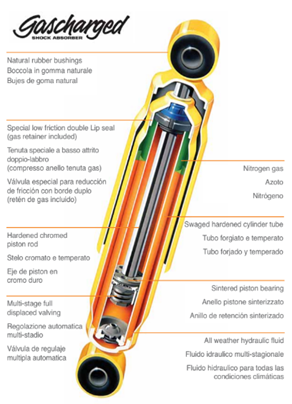
\includegraphics[scale=1]{amortecedorEE01.png}
		\caption[Amortecedor hidráulico tubo duplo]{Amortecedor hidráulico tubo duplo \cite{Cofap}} 
		\label{amortecedorEE01}
	\end{figure}

	Como ainda não foi possível acesso ao desenho específico do amortecedor, pode-se adotar a geometria cilíndrica para simulação. O modelo deve apresentar as dimensões específicas contidas no catálogo para que a malha se aproxime mais do modelo real. O modelo esperado da malha, pode ser observado na figura \ref{amortecedorEE02}:

	\begin{figure}[!h]
		\centering
		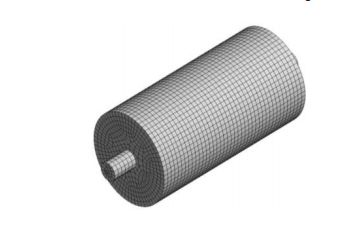
\includegraphics[scale=1]{amortecedorEE02.png}
		\caption[Malha do amortecedor com discretização do domínio]{Malha do amortecedor com discretização do domínio \cite{Neto}}
		\label{amortecedorEE02}
	\end{figure}

	Com a montagem da malha pode-se então iniciar as simulações de escoamento interno, com software ANSYS CFX  16.2, a partir do fornecimento dos diâmetros dos tubos e propriedades dos fluidos e materiais. A análise deve ser realizada em regime transiente, uma vez que as condições de contorno do escoamento variam com o tempo.
	
	Como resultados, o software pode fornecer distribuições de temperatura e velocidade no escoamento, em detrimento do número de Reynolds - coeficiente adimensional que classifica o escoamento em laminar ou turbulento, em função do diâmetro do duto, velocidade do escoamento, da viscosidade e da massa específica do fluido \cite{Pariona}.
	
	As figuras que seguem representam a evolução do comportamento em função do tempo, das distribuições de temperatura no plano do amortecedor. O mesmo gráfico pode variar para diferentes valores de velocidades de ensaio do amortecedor, variações de diâmetros dos tubos do amortecedor e diferentes fluidos de amortecimento.

	\begin{figure}[!h]
		\centering
		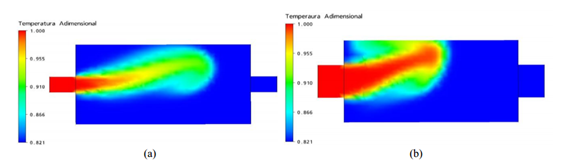
\includegraphics[scale=1]{amortecedorEE03.png}
		\caption[Distribuições de temperatura para um mesmo número de Reynolds e diferentes diâmetros de tubo]{Distribuições de temperatura para um mesmo número de Reynolds e diferentes diâmetros de tubo \cite{Neto}} 
		\label{amortecedorEE03}
	\end{figure}

	A partir de várias análises como a apresentada, poderão ser obtidas conclusões acerca do desempenho do amortecedor a partir do comportamento do fluido contido em seu interior, o que torna este estudo viável para o projeto em curso. Um dos parâmetros de interesse é a determinação da temperatura do fluido durante o ensaio, uma vez que a temperatura medida será a da carcaça. Assim, a finalidade do estudo é obter um gradiente de temperatura para o ensaio de amortecedores, que nos dê como resultado a temperatura do fluido naquele instante.

\newpage
\subsection{Ponto de Controle III}
\subsubsection{Ensaio com o Protótipo Adaptado da Bancada}
	
	Para realizar os primeiros ensaios, diante da impossibilidade, até o presente momento, de testes na bancada real proposta pelo grupo, foi construído um protótipo que simulou a situação do teste proposto neste projeto. Trata-se de uma bancada adaptada, composta por motor de indução trifásico, caixa de redução e amortecedor, todos parafusados em uma base de madeira. 
	
	Inicialmente, testou-se um amortecedor de motocicleta, tanto para comprovar a variedade de possibilidades de testes que a estrutura adaptada e o conjunto motor-inversor dimensionado oferecem, juntamente com a caixa de redução, quanto para assegurar que a base de madeira suportaria as forças nela exercidas. Em um segundo momento, foi então testado o amortecedor traseiro GL12380 Cofap, do veículo \textit{Fiat Strada}.

	O objetivo destes testes foi garantir o bom funcionamento do sistema, pois, ao utilizar apenas dois sistemas de transmissão (do motor para a caixa de redução de 5/8 e da própria caixa de 1/12), enquanto a proposta inicial objetivou utilizar além desses, dois outros sistemas de redução, já foi possível se comprovar a eficiência de excitação do sistema. 
	
	O esquema abaixo mostra o sistema de transmissão motor-redutor considerado, no qual a polia do motor tem como raio 3,75 cm e a polia da caixa de redução tem raio 6 cm.

	\begin{figure}[!hbtp]
		\centering
		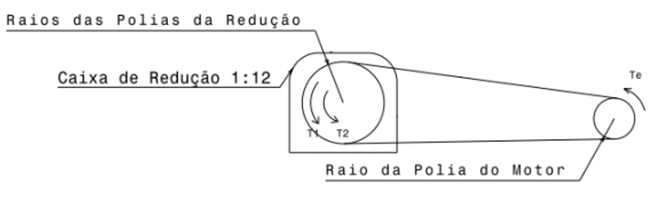
\includegraphics[scale=0.8]{ene1.png}
		\caption{Esboço do sistema de transmissão motor-redutor.} 
		\label{ene1}
	\end{figure}

\subsubsection{Teste com Amortecedor de Motocicleta}
	
	A partir do sistema de transmissão mostrado no item anterior, como a caixa de redução é coaxial, foi acoplado no eixo do lado oposto um disco de raio 9 cm e nele foi acoplado o amortecedor a ser testado. Essa conexão do disco com o amortecedor, representada na Figura \ref{ene2}, foi feita através de um parafuso e uma bucha fabricada no galpão da UnB – Faculdade do Gama, de forma a ter a flexibilidade necessária para acompanhar a rotação do disco. 
	
	A montagem do sistema, contemplando o motor, a caixa de redução e o amortecedor também segue representada na Figura \ref{ene3}.

	\begin{figure}[!hbtp]
		\centering
		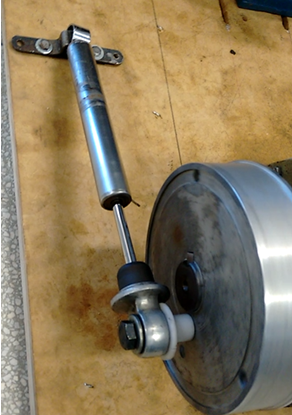
\includegraphics[scale=0.8]{ene2.png}
		\caption{Acoplamento do amortecedor de moto ao disco da caixa de redução.} 
		\label{ene2}
	\end{figure}

	\begin{figure}[!hbtp]
		\centering
		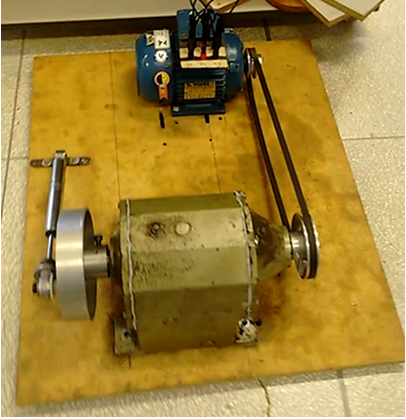
\includegraphics[scale=0.8]{ene3.png}
		\caption{Sistema montado.} 
		\label{ene3}
	\end{figure}

	Obteve-se êxito no teste em questão, visto que o sistema teve um comportamento totalmente eficiente, conseguindo atender o objetivo proposto. O amortecedor foi testado durante 8 minutos, sendo que houve a possibilidade de variação de três velocidades (300, 500 e 900 rpm) através do inversor de frequência e das chaves seletoras, mostrando-se seguro durante todo o tempo. Como a estrutura mostrou-se segura e a montagem permitiu que o teste fosse realizado conforme as exigências propostas, seguiu-se então para o outro teste com o amortecedor que será de fato testado na bancada final.

\subsubsection{Teste com Amortecedor de Veículo \textit{Fiat Strada}}
	
	Foram feitos testes com o amortecedor do veículo \textit{Fiat Strada}, o qual se encaixa na proposta da bancada projetada pelo grupo. Segue representada na Figura \ref{ene4} o acoplamento de tal amortecedor ao disco da caixa de redução. A outra extremidade do amortecedor foi fixada na base de madeira por meio de um mancal, um parafuso e uma bucha, representados na Figura \ref{ene5}.

	\begin{figure}[!hbtp]
		\centering
		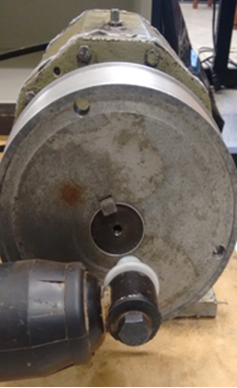
\includegraphics[scale=0.7]{ene4.png}
		\caption{Acoplamento do amortecedor ao disco da caixa de redução.} 
		\label{ene4}
	\end{figure}

	\begin{figure}[!hbtp]
		\centering
		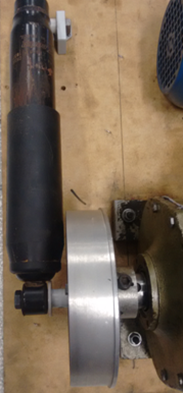
\includegraphics[scale=0.7]{ene5.png}
		\caption{Acoplamento do amortecedor ao sistema.} 
		\label{ene5}
	\end{figure}

	O sistema completo (motor-redutor-amortecedor) pode ser visualizado na Figura \ref{ene6}, onde se tem a transmissão por polias e correia do motor para o redutor, assim como o acoplamento do amortecedor na saída da caixa de redução. Como já mencionado, no sistema de redução por polias existente entre o motor e o redutor, tem-se uma razão redução de velocidades de 5/8. No ponto onde se encontra o disco e o amortecedor acoplado, tem-se razão de 1/12. 
	
	Portanto, no ponto de excitação direta do amortecedor, há diminuição de velocidade e aumento de torque, de grande valia para a execução de compressão e expansão do mesmo.

	\begin{figure}[!hbtp]
		\centering
		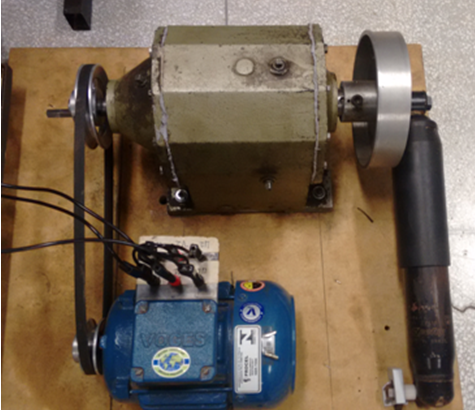
\includegraphics[scale=0.7]{ene6.png}
		\caption{Sistema de teste adaptado para o amortecedor de veículo \textit{Fiat Strada}.} 
		\label{ene6}
	\end{figure}

	O circuito elétrico montado faz a conexão de 3 fusíveis com o inversor de frequência, que por sua vez é conectado ao motor de indução trifásico. Foram usadas chaves seletoras para a escolha das velocidades programadas, pela lógica binária apresentada anteriormente na Figura \ref{posicaoChave}.  
	
	Além da proteção externa que os fusíveis proporcionam, o inversor de frequência oferece ao sistema proteção padrão de sobrecarga do motor, além de permitir a programação de proteção de sobrecorrente pela função \textit{“Hold de Rampa”}, que evita o tombamento do motor durante sobrecarga de torque na aceleração ou desaceleração. Quando programada essa função, se a corrente do motor ultrapassar o valor pré-ajustado durante a aceleração ou desaceleração, a velocidade não será mais aumentada (aceleração) ou diminuída (desaceleração). Assim, somente quando a corrente do motor atingir um valor abaixo do ajustado, o motor volta a acelerar ou desacelerar.
	
	A Figura \ref{ene7} mostra o sistema completo, desde a alimentação elétrica do sistema até o protótipo construído para o ensaio de excitação do amortecedor.

	\begin{figure}[!hbtp]
		\centering
		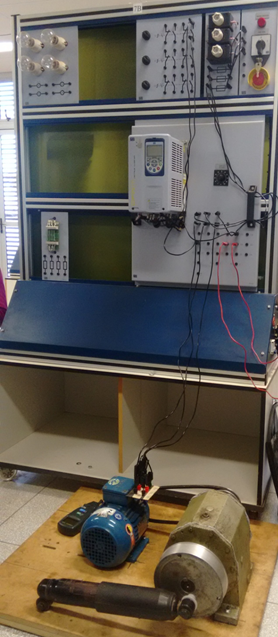
\includegraphics[scale=0.7]{ene7.png}
		\caption{Sistema completo de teste adaptado para o amortecedor de veículo \textit{Fiat Strada}.} 
		\label{ene7}
	\end{figure}

	A estrutura nos forneceu a possibilidade de excitar o amortecedor através de um curso de 5,5 cm, com as velocidades citadas na Figura abaixo e obter os seguintes resultados.

	\begin{figure}[!hbtp]
		\centering
		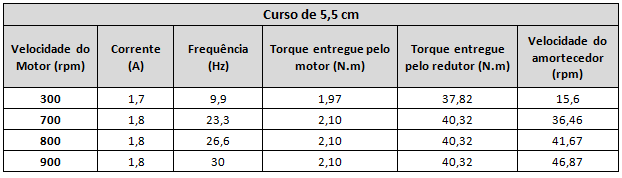
\includegraphics[scale=0.9]{ene8.png}
		\caption{Resultados obtidos no teste do amortecedor de veículo \textit{Fiat Strada}.} 
		\label{ene8}
	\end{figure}

	As velocidades testadas no motor foram programadas a fim de se estabelecer uma rampa de aceleração, começando por uma velocidade baixa (de 300 rpm), tendo a opção de retornar a essa velocidade antes de desligar o motor, com o auxílio das chaves seletoras. Ainda foi estabelecida a partida do motor por rampa de aceleração quando se programou o parâmetro “Habilita Geral” do inversor de frequência, que permite essa função. Além disso, como o motor utilizado é autoventilado, foram testadas velocidades relativamente baixas, para se comprovar que o torque exigido pela carga será atendido mesmo em situações consideradas críticas para o motor, previamente calculadas.

\subsubsection{Principais Contribuições da Equipe de Energia para o Projeto}
	
	Foi realizado por parte da Equipe de Energia todo o dimensionamento necessário ao acionamento do sistema, depois foram feitos todos os testes necessários com o conjunto motor-inversor e com a caixa de redução, que comprovaram na prática os dados calculados e garantiram o funcionamento do sistema. 
	
	Dadas as condições, foi construída por duas integrantes da Equipe da Energia uma estrutura adaptada, na qual se conseguiu testar os amortecedores de motocicleta e de veículo \textit{Fiat Strada}, simulando a situação mais próxima à real possível do teste proposto, segundo as condições impostas pelo grupo. Para a construção de tal estrutura, utilizou-se de materiais cedidos por terceiros e de outros fabricados no Galpão da Faculdade do Gama FGA, como por exemplo os pontos de apoio do amortecedor. 
	
	Pela impossibilidade de gastos extras, que pudessem ir além dos estabelecidos para a bancada real, os meios de escolha de materiais para a construção da estrutura adaptada foram limitados. Apesar de tal estrutura não contemplar o sistema biela-manivela, que existirá na bancada real, pois o mesmo está em fase de construção, o conjunto motor-inversor juntamente com a caixa de redução mostrou efetivamente que, assim como proposto, os testes dos amortecedores automotivos são executáveis com eficiência e segurança pelo sistema de alimentação dimensionado.


\subsubsection{Considerações Finais da Equipe de Energia}

	Todos os testes realizados com o motor de indução trifásico, o inversor de frequência, a caixa de redução e os amortecedores foram de extrema importância tanto para o entendimento do funcionamento do sistema quanto para fins comprobatórios de que o sistema de acionamento dos testes de amortecedores propostos pelo projeto em questão é viável, eficaz e atende aos requisitos impostos. Como supracitado, apesar dos imprevistos ocorridos ao desenvolver do projeto, como falta de elementos necessários aos testes da bancada real proposta, foi possível, até então, de forma adaptada, testar os amortecedores de motocicleta e de um \textit{Fiat Strada} e comprovar a capacidade do sistema de acionamento.
	

